\documentclass[12pt]{article}
\usepackage[english]{babel}
\usepackage[T1]{fontenc}
\usepackage{color}
\usepackage{fancyvrb}
\usepackage{hyperref}
\usepackage[procnames]{listings}
\usepackage{blindtext}
\usepackage{graphicx}
\usepackage{float}
\usepackage{caption}
\captionsetup[table]{labelsep=period}
\usepackage{changepage}
\usepackage{authblk}
\usepackage{titling}

\setlength{\droptitle}{-8em} 

\begin{document}
		
\title{Reducing noise in protein multialignments}
\posttitle{\par\end{center}\vspace{-1em}}
\author{Marina Herrera Sarrias}
\affil{Department of Mathematics, Stockholm University}
\affil{mherrera@kth.se}
\date{January 6, 2019}                    %% if you don't need date to appear
\maketitle

\section{Abstract}

In this research a noise-reduction method is implemented in protein multialigments to evaluate its impact on phylogenic inference. The data used in this project is a reduced data set from the  original data used by the creators of \href{http://trimal.cgenomics.org}{TrimAI}. To test the data the program \href{http://fastphylo.sourceforge.net/}{fastprot} was used to obtain the distance matrices and \href{http://fastphylo.sourceforge.net/}{fnj} to infer a phylogenic tree for each alignment. The Python package \href{https://dendropy.org/}{DendroPy} was used to measure the symmetric distance between the inferred tree (of the original and noise reduced alignment) and the reference tree. The results obtained showed that the symmetric difference between the reference tree and the noise reduced tree is in most of the cases lower than in the case of the symmetric distance between the reference tree and the original inferred tree. Although, in most of the cases the method applied did not make any change between the noise reduced inferred tree and the original inferred tree. This study focuses in determining whether the noise reduction makes any effect in the symmetric distance calculation.

\section{Introduction}
Phylogenetis is the study of the evolutionary relationship among a group of organisms. There is a strong relationship between the studies of phylogenetics and sequences analysis, if two sequences found in two  different organisms are very similar we can then assume that they have derived from a common ancestor. When a multiple sequence alignment is performed it compares sequences in order to find similarities, it will firstly align the most similar pairs followed by the most distant pairs. The sequences alignment explains which positions are conserved from the ancestor sequence. Gaps in the alignments represent mutations therefore, the greater number of differences the more possible kind of mutations there will be.\\

Phylogenetic trees illustrate this relationship between organisms. The leaves of the tree represent the sequences, the nodes the relationship between them and the length of the branches, the number of changes that occurred in the sequences before the next level of separation. Trees could differ depending on the method used to construct them and there is not such as "best tree" whether there is a "good tree". The topology refers to the branching pattern of the tree, symmetry and asymmetry of a tree makes reference to how balanced or imbalanced the tree is, if the sequences(taxa) are evenly distributed among the clades the tree is balanced, otherwise is imbalanced. The objective of this project is to determine, whether it is worthwhile to use multialignment noise reduction in order to infeer a tree with fewer changes, and therefore a lower symmetric distance.\\

The reduced data set used in this project is composed by six different sub-directories, each sub-directory contains a reference tree and 300 alignments created by evolving sequences along the reference tree. Each pair of sub-directories present an average amount of mutations of 0.5, 1.0 and 2.0 per sequence site. Also, per each mutation rate there is one symmetric reference tree and one asymmetric reference tree. \\

In this project, the implemented noise-reduction method evaluates a multialigment column as noisy if there are more than $50\%$ indels, at least $50\%$ of the amino acids are unique and non of the amino acids appear more than twice. Each column takes the form of a sequence of amino acids given a position of the aligned sequences. \\

The results of the study showed that in most of the cases the applied noise reduction method did not have any effect on the symmetric distance calculation. Although it did showed a better performance in comparison with the original inferred tree, specially for those trees with higher average mutation rate.


\section{Results and Discussion}
 
After verifying the correct functionality of the program and processing the six data sets a frequency table of the six possible symmetric distance scenarios was compiled (Table \ref{table:freqtable}).\\

In most of the cases the original tree and the noise reduced  alignment tree are the same, indicating that the method applied had no effect in most of the alignments. In case for which the effect was not the same between the original and noise reduced inferred tree, the effect of reducing noise in the alignments makes the new noise reduced data to have a smaller symmetric distance with the reference tree, while there are fewer cases in which the effect is the opposite.\\

The reference tree was recovered with a greater frequency when the tree was  symmetric and the average amount of mutations per sequence site was lower. From this, it can be understand that the symmetric difference is equal to 0. According to the frequency values, the reference tree was recovered 3 times by the noise reduced tree  while it was recovered 5 times by the original multi-alignment inferred tree. \\

Table \ref{table:statistics} gives statistical information about the six data sets. Both inferred trees (original and noise reduced) take nearly the same minimum (not taking into account distances of 0), maximum, mean and median values. 


\begin{table}[H]

	\caption{Frequencies of  the symmetric distances of the original and reduced newick trees compared to the reference tree.}
	\begin{adjustwidth}{-2cm}{}
	\small\addtolength{\tabcolsep}{-3pt}
	\begin{tabular}{l|c|c|c|c|c|c|l}
		\cline{2-7}
		\textbf{} & \multicolumn{1}{l|}{Asymm\_0.5} & \multicolumn{1}{l|}{Asymm\_1.0} & \multicolumn{1}{l|}{Asymm\_ 2.0} & \multicolumn{1}{l|}{Symm\_0.5} & \multicolumn{1}{l|}{Symm\_1.0} & \multicolumn{1}{l|}{Symm\_2.0} &  \\ \cline{1-7}
		\multicolumn{1}{|l|}{Original \textgreater Reduced} & 45 & 60 & 79 & 44 & 59 & 83 &  \\ \cline{1-7}
		\multicolumn{1}{|l|}{Original \textless Reduced} & 48 & 54 & 45 & 28 & 36 & 54 &  \\ \cline{1-7}
		\multicolumn{1}{|l|}{Original = Reduced} & 206 & 186 & 176 & 214 & 201 & 162 &  \\ \cline{1-7}
		\multicolumn{1}{|l|}{Original = 0} & 0 & 0 & 0 & 4 & 1 & 0 &  \\ \cline{1-7}
		\multicolumn{1}{|l|}{Reduced = 0} & 0 & 0 & 0 & 2 & 1 & 0 &  \\ \cline{1-7}
		\multicolumn{1}{|l|}{Original \& Red = 0} & 1 & 0 & 0 & 8 & 2 & 1 &  \\ \cline{1-7}
		\multicolumn{1}{|l|}{\textbf{Total}} & 300 & 300 & 300 & 300 & 300 & 300 &  \\ \cline{1-7}
	\end{tabular}
\label{table:freqtable}
 \end{adjustwidth}
\end{table}

\begin{table}[H]
	\caption{Data sets statistics referring to the symmetric distance of the original and reduced newick trees with the reference tree.}	 
	\begin{adjustwidth}{-1cm}{}   
	\small\addtolength{\tabcolsep}{-3pt}
	\begin{tabular}{lcccccccc}
		\cline{2-9}
		\multicolumn{1}{c|}{\textbf{}} & \multicolumn{2}{c|}{Minimum} & \multicolumn{2}{c|}{Maximum} & \multicolumn{2}{c|}{Mean} & \multicolumn{2}{c|}{Median} \\ \cline{2-9} 
		\multicolumn{1}{l|}{\textbf{}} & \multicolumn{1}{l|}{Original} & \multicolumn{1}{l|}{Reduced} & \multicolumn{1}{l|}{Original} & \multicolumn{1}{l|}{Reduced} & \multicolumn{1}{l|}{Original} & \multicolumn{1}{l|}{Reduced} & \multicolumn{1}{l|}{Original} & \multicolumn{1}{l|}{Reduced} \\ \hline
		\multicolumn{1}{|l|}{Asymmetric 0.5} & \multicolumn{1}{c|}{2} & \multicolumn{1}{c|}{2} & \multicolumn{1}{c|}{18} & \multicolumn{1}{c|}{18} & \multicolumn{1}{c|}{7.63} & \multicolumn{1}{c|}{7.62} & \multicolumn{1}{c|}{8} & \multicolumn{1}{c|}{8} \\ \hline
		\multicolumn{1}{|l|}{Asymmetric 1.0} & \multicolumn{1}{c|}{2} & \multicolumn{1}{c|}{2} & \multicolumn{1}{c|}{18} & \multicolumn{1}{c|}{18} & \multicolumn{1}{c|}{9.43} & \multicolumn{1}{c|}{9.39} & \multicolumn{1}{c|}{10} & \multicolumn{1}{c|}{10} \\ \hline
		\multicolumn{1}{|l|}{Asymmetric 2.0} & \multicolumn{1}{c|}{4} & \multicolumn{1}{c|}{4} & \multicolumn{1}{c|}{22} & \multicolumn{1}{c|}{20} & \multicolumn{1}{c|}{12.34} & \multicolumn{1}{c|}{11.99} & \multicolumn{1}{c|}{12} & \multicolumn{1}{c|}{12} \\ \hline
		\multicolumn{1}{|l|}{Symmetric 0.5} & \multicolumn{1}{c|}{2} & \multicolumn{1}{c|}{2} & \multicolumn{1}{c|}{10} & \multicolumn{1}{c|}{10} & \multicolumn{1}{c|}{4.66} & \multicolumn{1}{c|}{4.55} & \multicolumn{1}{c|}{4} & \multicolumn{1}{c|}{4} \\ \hline
		\multicolumn{1}{|l|}{Symmetric 1.0} & \multicolumn{1}{c|}{2} & \multicolumn{1}{c|}{2} & \multicolumn{1}{c|}{12} & \multicolumn{1}{c|}{12} & \multicolumn{1}{c|}{6.23} & \multicolumn{1}{c|}{6.05} & \multicolumn{1}{c|}{6} & \multicolumn{1}{c|}{6} \\ \hline
		\multicolumn{1}{|l|}{Symmetric 2.0} & \multicolumn{1}{c|}{2} & \multicolumn{1}{c|}{2} & \multicolumn{1}{c|}{16} & \multicolumn{1}{c|}{16} & \multicolumn{1}{c|}{8.91} & \multicolumn{1}{c|}{8.65} & \multicolumn{1}{c|}{8} & \multicolumn{1}{c|}{8} \\ \hline
		& \multicolumn{1}{l}{} & \multicolumn{1}{l}{} & \multicolumn{1}{l}{} & \multicolumn{1}{l}{} & \multicolumn{1}{l}{} & \multicolumn{1}{l}{} & \multicolumn{1}{l}{} & \multicolumn{1}{l}{}
	\end{tabular}
	\label{table:statistics}
	 \end{adjustwidth}
\end{table}

The noise reduction performance was slightly higher on the symmetric sets compared to the asymmetric (Table \ref{table:averg}) , the noise reduction average was observed to increase with the average mutation rate. 



\begin{table}[H]
	\centering
	\small\addtolength{\tabcolsep}{-2pt}
	\caption{Average noise reduction performed per data set}
	\begin{tabular}{l|c|l}
		\cline{2-2}
		\textbf{} & \multicolumn{1}{l|}{Average Noise Reduction} &  \\ \cline{1-2}
		\multicolumn{1}{|l|}{Asymmetric 0.5} & 0.146 &  \\ \cline{1-2}
		\multicolumn{1}{|l|}{Asymmetric 1.0} & 0.199 &  \\ \cline{1-2}
		\multicolumn{1}{|l|}{Asymmetric 2.0} & 0.252 &  \\ \cline{1-2}
		\multicolumn{1}{|l|}{Symmetric 0.5} & 0.172 &  \\ \cline{1-2}
		\multicolumn{1}{|l|}{Symmetric 1.0} & 0.221 &  \\ \cline{1-2}
		\multicolumn{1}{|l|}{Symmetric 2.0} & 0.282 &  \\ \cline{1-2}
	\end{tabular}

\label{table:averg}
\end{table}


\section{Methods and Materials}
Three different major tasks were first developed separately, and later joined together to consolidate the program and conduct an exploratory data analysis. The individual scripts were initially tested on the experimental data and control cases and then merged in a single script to later run the program with the fixed data set.\\

\clearpage

A \href{https://github.com/msarrias/protein_multial_noise_reduction}{Github repository} was created in order to control the program's version. The Laboratory notebook was created using a Jupyter notebook Markdown and later compiled into a HTML file, which can be found on the \href{https://github.com/msarrias/protein_multial_noise_reduction/tree/master/results}{Github repository}. This notebook contains all details regarding the development of the current project.\\

Following the \href{https://journals.plos.org/ploscompbiol/article?id=10.1371/journal.pcbi.1000424#s6}{course centerpiece guideline}, controls were introduced along the project as well error handling. When an error occurs the program aborts and prints a message to standard error. All standard-in files are read by robust libraries. 
%The program do not creates a temporary name for the output file.%
Moreover, a sub-directory containing a subset of the fixed data set was created in order to test the program, controls for different scenarios were also introduced to ensure the program functionality. No input is required for testing the data, neither for running the main program.\\

\subsection{Running: run\_program.py}

The python script run\_program.py performs all the required tasks of the different stages of this project:

\begin{enumerate}
	\item Reduce protein multialignment noise: 
The program first takes an alignment from standard-in, filters the columns and writes a new file containing the noise reduced multi-alignment. 
In order to illustrate the functionality of the program,   \href{http://doua.prabi.fr/software/seaview}{Seaview} was used as a graphical interface for the following example.\\

 As shown below, the original alignment before (Figure \ref{fig:al_1} ) and after performing noise reduction (Figure \ref{fig:al_2}). In this particular case the reduced noise  represented a $17.08\%$ of the original sequence.

\begin{figure}[H]
	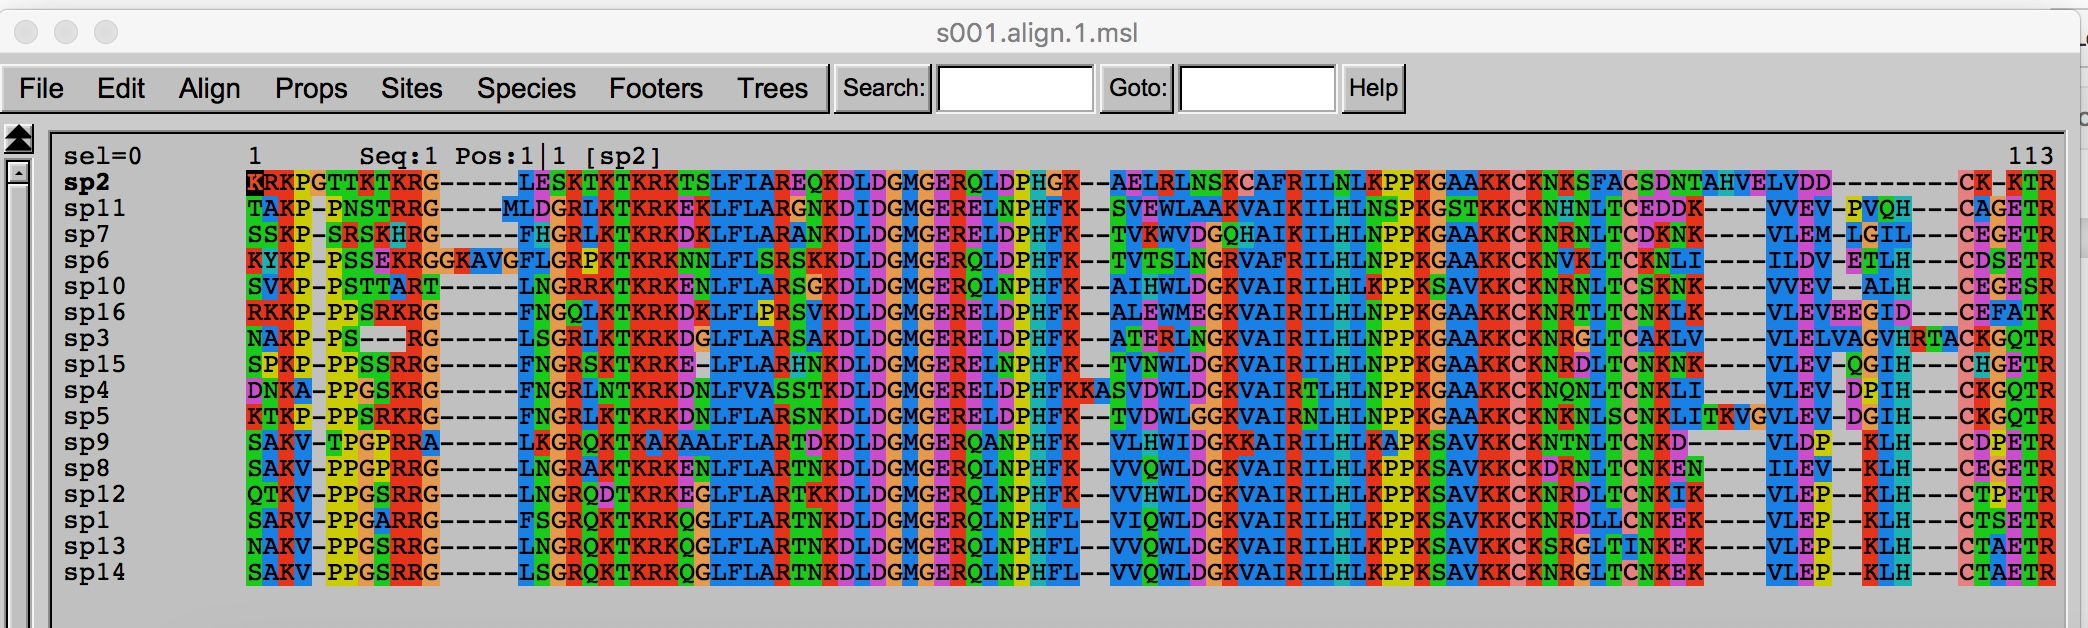
\includegraphics[width=\linewidth]{labnotes2.png}
	\caption{Original s001.align.1.msl}
	\label{fig:al_1}
\end{figure}

\begin{figure}[H]
	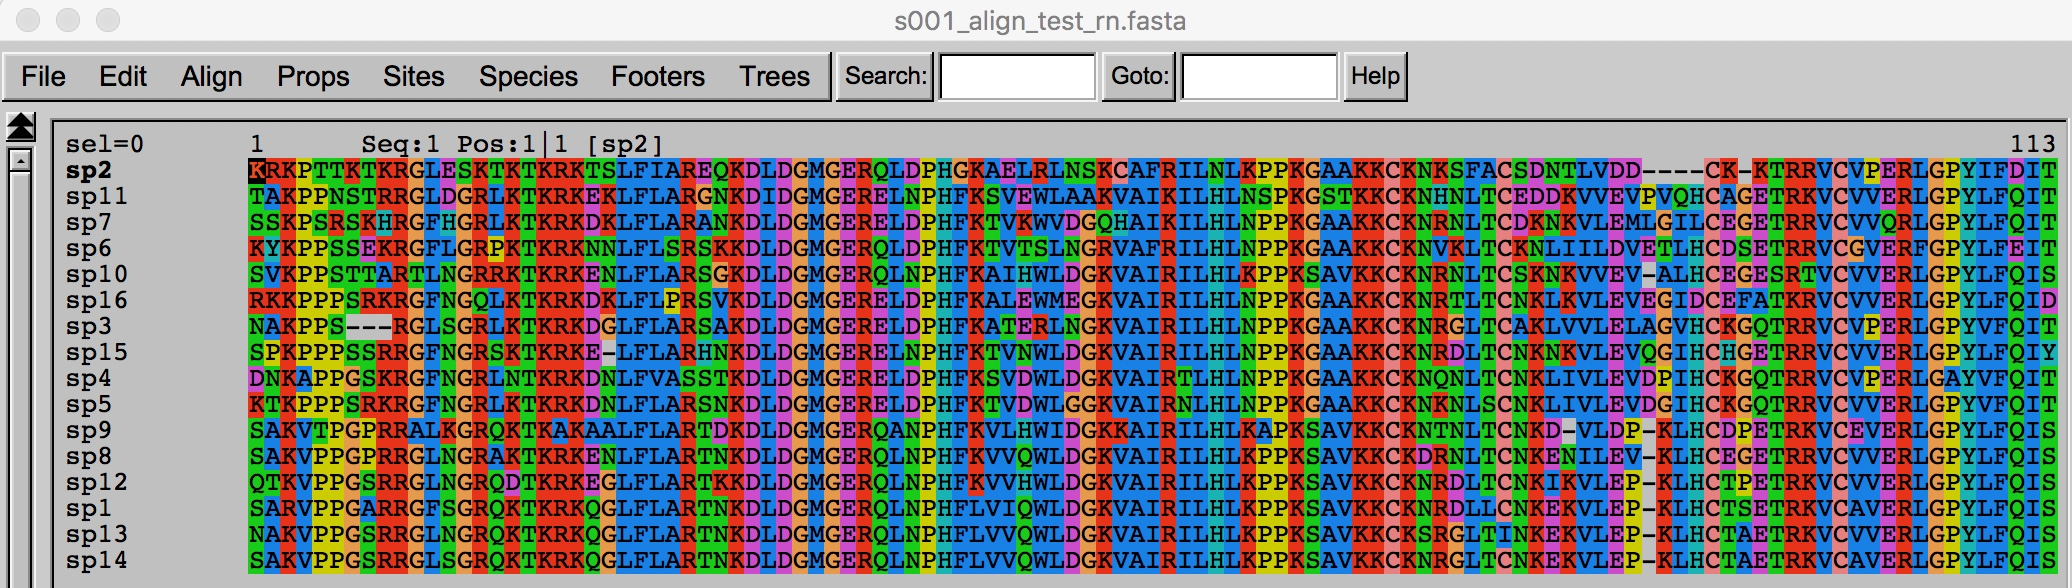
\includegraphics[width=\linewidth]{labnotes_1.png}
	\caption{s001.align.1.msl after noise reduction}
	\label{fig:al_2}
\end{figure}
	
	\item Generate phylogenetic trees:
 On the second stage, the program pars through all the alignments available in the data directory (original and noise reduced), and using the  \href{http://fastphylo.sourceforge.net/}{fastphylo} programs (fastprot and fnj) computes a distance matrix and generate a phylogenetic tree per alignment. In order to accomplish this task the program uses a sub-process to pipe the matrix creation and generate the tree. As the symmetric distance (computed in next stage) only requires the tree's topology it will not be necessary to compute the branch length information.  \\
 
  Following the s001.align.1.msl alignment example both, the noise reduced and original alignment have the same phylogenetic tree shown in Figure \ref{fig:reducedoriginaltree} while the reference tree is represented by  Figure \ref{fig:referencetree}.
  
\begin{figure}[H]
	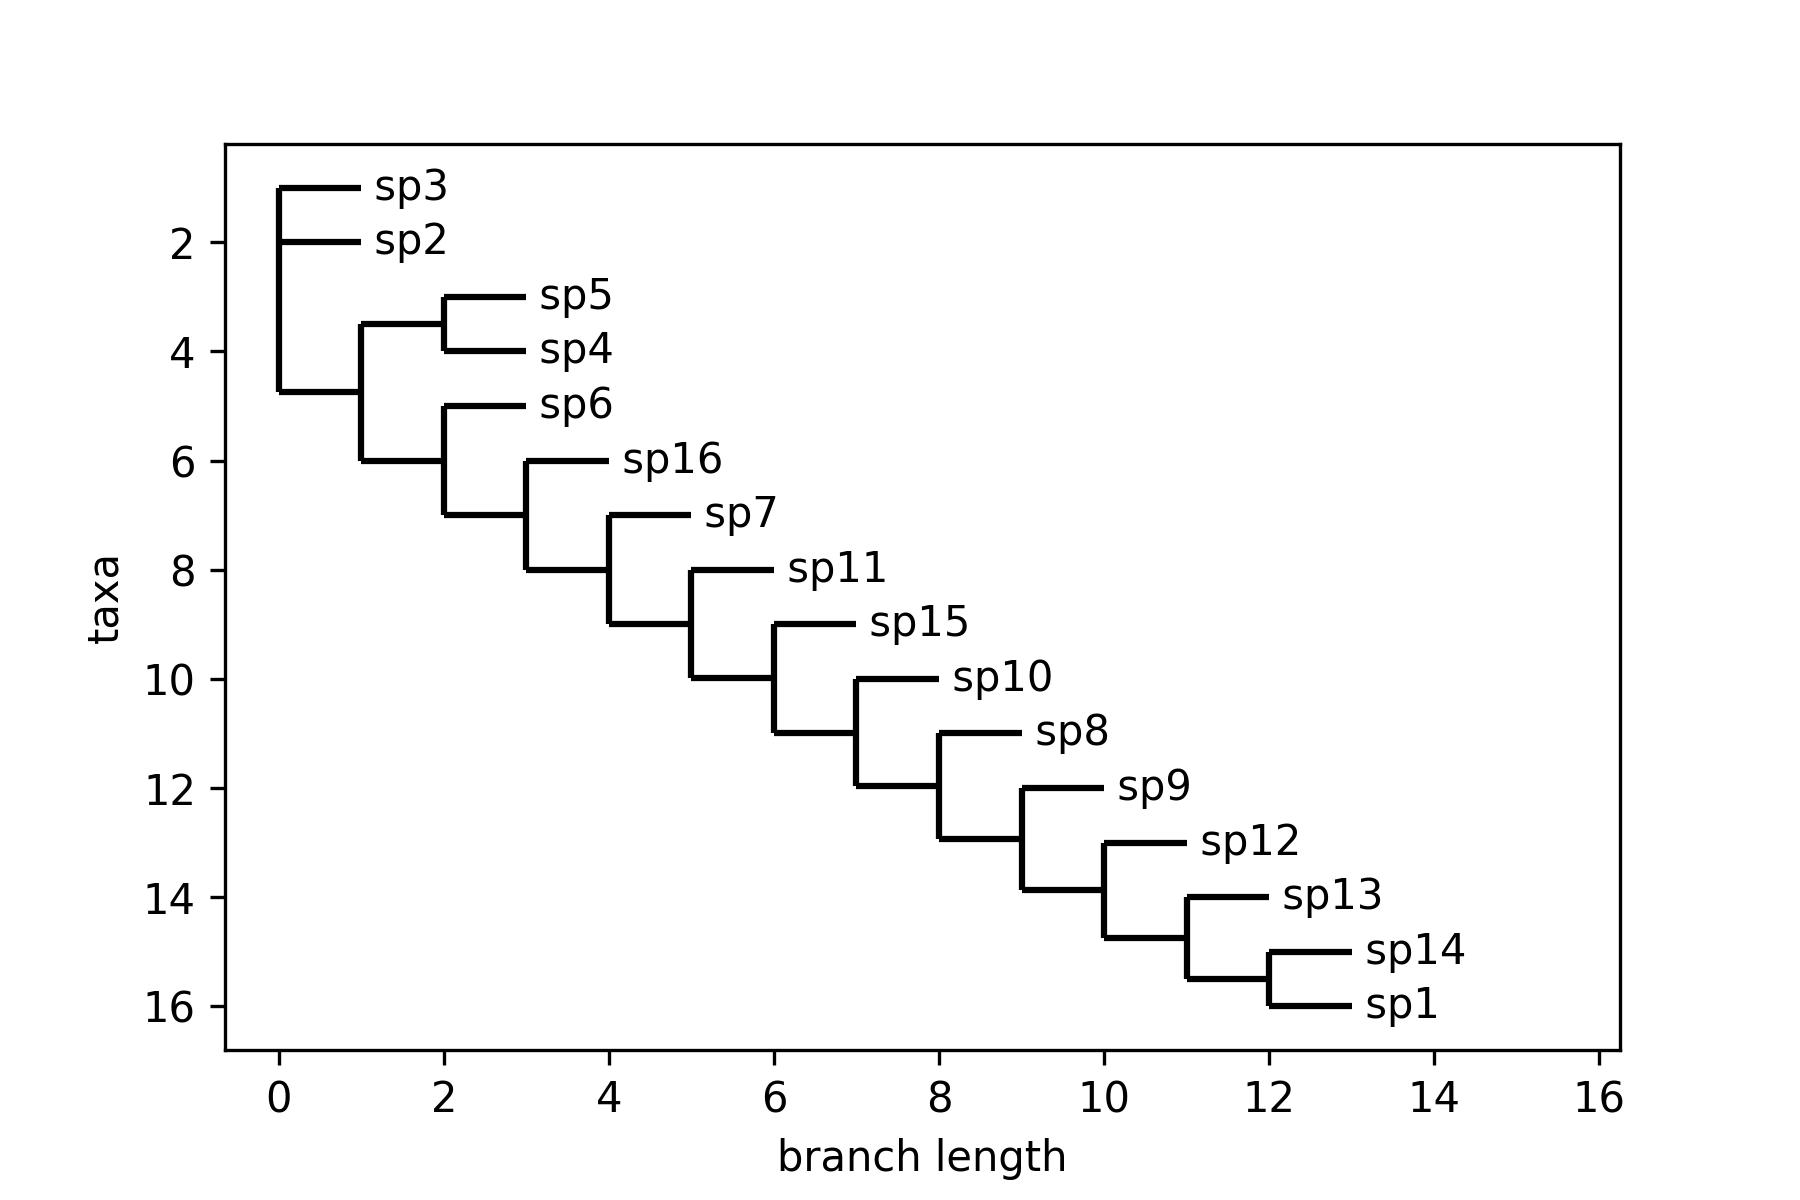
\includegraphics[width=.9\linewidth]{reduced_original.png}
	\caption{s001.align.1.msl original and noise reduced tree}
	\label{fig:reducedoriginaltree}
\end{figure}

\begin{figure}[H]
	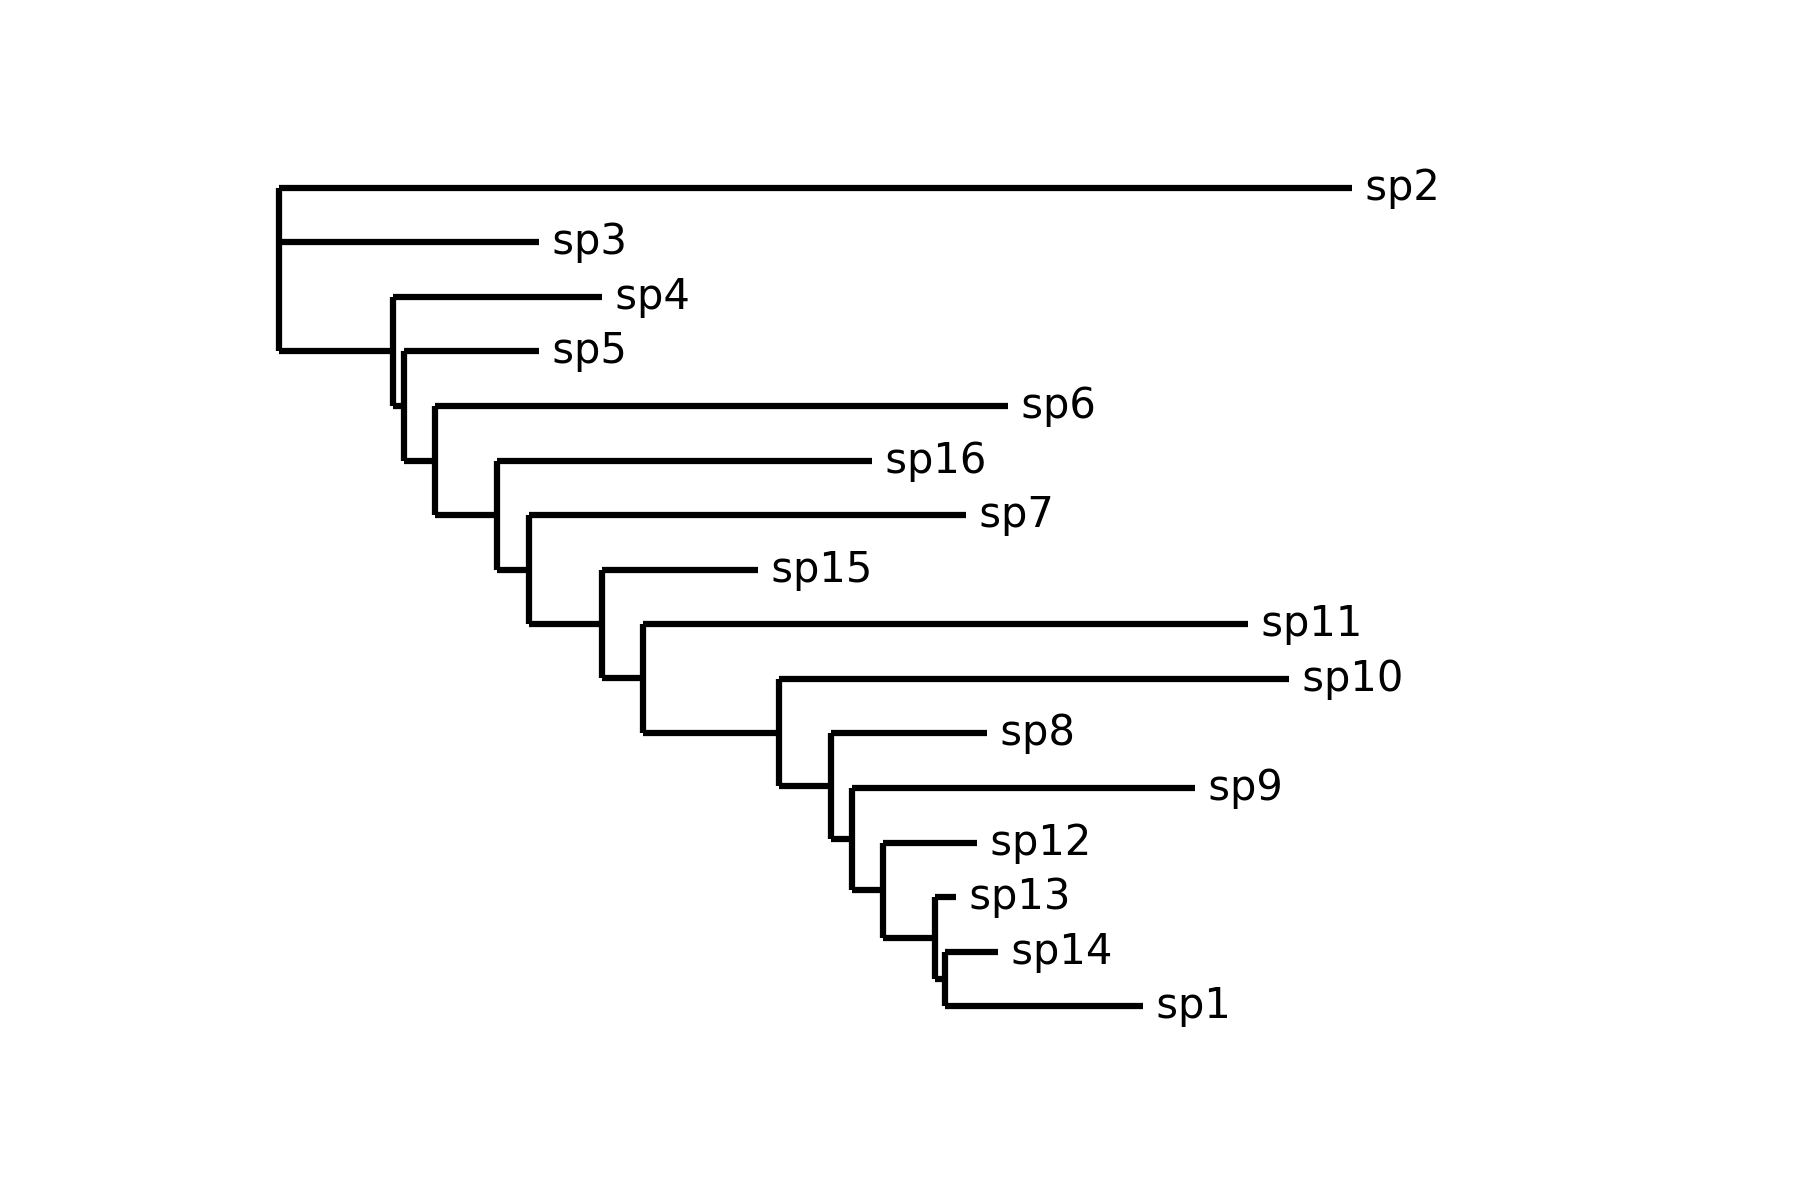
\includegraphics[width=.9\linewidth]{reference.png}
	\caption{asymmetric\_0.5.tree reference tree}
	\label{fig:referencetree}
\end{figure}

\item Compute trees distances: Finally, the program computes the symmetric distance between the reference tree and both, original and noise reduced tree using the python's module \href{https://dendropy.org/}{Dendropy}. The symmetric distance is a count of how many partitions are between the two trees, that are present in one tree but not in the other. Following the s001.align.1.msl, alignment example, as both the original tree and noise reduced tree are the same the distance with the reference tree will be therefore the same, in this case 4.  
\end{enumerate}

\subsection{run\_program.py: Error handling and Control cases }

The script run\_program.py will abort if any of the following cases occur:
\begin{itemize}
	\item There is an input introduction when executing the program.
	\item The data directory is empty.
	\item The data sub-directories are empty. (e.g asymmetric\_0.5).
	\item Any of the standard-in file (.msl,.tree) is empty.
	\item All the columns in the alignment are noisy. 
\end{itemize}
On the other hand, the program will  print a warning message but will not abort processing if:
\begin{itemize}
	\item The alignment do not have noisy columns.
	\item The noise reduction rate is greater than 0.5 times the original alignment.
\end{itemize}

All of the control files used for testing the accuracy of this script can be found in the results directory of  \href{https://github.com/msarrias/protein_multial_noise_reduction/tree/master/results/control_case_data}{Github repository}, in which a file for each case above-mentioned can be found.
\end{document}
